% !TEX options=--shell-escape

\documentclass[10pt]{beamer}

\usepackage[T1]{fontenc}
\usepackage{beramono}

\usepackage{anyfontsize}
\usepackage{booktabs}
\usepackage{etoolbox}
\usepackage{hyperref}
\usepackage{setspace}
\usepackage{tcolorbox}
\usepackage{texlogos}
\usepackage{xcolor}
\usepackage{xspace}
\usepackage{graphicx}

\usetheme{metropolis}
\usepackage{appendixnumberbeamer}

\newcommand\cpp[1]{\cpluspluslogo #1}
\newcommand\mono[1]{\texttt{\footnotesize{\detokenize{#1}}}\xspace}
\newcommand\pybind{\mono{pybind11}}
\newcommand\codeskip{\\\vspace*{0.5em}}
\newcommand\darrow{\parbox{3cm}{\centering$\downarrow$}\smallskip}
\newcommand\supertiny{\fontsize{3}{3}\selectfont}
\newcommand\smaller{\fontsize{6}{6}\selectfont}

\definecolor{urlcolor}{rgb}{0.75,0.45,0.15}
\renewcommand\UrlFont{\footnotesize\ttfamily\color{urlcolor}}

\definecolor{lgreen}{rgb}{0.8,0.9,0.8}
\definecolor{lred}{rgb}{0.9,0.8,0.8}
\definecolor{lgrey}{rgb}{0.6,0.6,0.6}
\definecolor{lblue}{rgb}{0.8,0.8,0.9}

\definecolor{dgreen}{rgb}{0.2,0.6,0.2}
\definecolor{dred}{rgb}{0.6,0.2,0.2}

\newcommand\hlbox[2]{\setlength{\fboxsep}{0pt}\colorbox{#1}{#2}}
\newcommand\hlcode[1]{\hlbox{lgreen}{\detokenize{#1}}}
\newcommand\hlcodealt[1]{\hlbox{lblue}{\detokenize{#1}}}
\newcommand\dimcode[1]{\hlbox{lgrey}{\detokenize{#1}}}

\usepackage{minted}
\usemintedstyle{trac}
\newminted{cpp}{autogobble,escapeinside=@@,fontsize=\footnotesize}
\newminted{python}{autogobble,escapeinside=@@,fontsize=\footnotesize}
\newminted{sh}{autogobble,escapeinside=@@,fontsize=\footnotesize}
\BeforeBeginEnvironment{minted}{
    \begin{tcolorbox}[colback=black!3!white,colframe=black!16!white,boxrule=0.3mm]
    }
\AfterEndEnvironment{minted}{\end{tcolorbox}}
\AtBeginEnvironment{minted}{\setstretch{1.2}}

\title{Python Tutorial}
\subtitle{CS-328 Numerical Methods for Visual Computing}
\date{September 20, 2017}
\author{Tizian Zeltner\\
Jan Bednarik}
%\institute{Susquehanna International Group\\
%[6\baselineskip]{euro\textbf{python} 2017}}

\begin{document}

\maketitle


%%%%%%%%%%%%%%%%%%%%%%%%%%%%%%%%%%%%%%%%%%%%%%%%%%%%%%%%%%%%%%%%%%%%%%%%%%%%%
%%%%%%%%%%%%%%%%%%%%%%%%%%%%%%%%%%%%%%%%%%%%%%%%%%%%%%%%%%%%%%%%%%%%%%%%%%%%%
\section{Introduction}

%%%%%%%%%%%%%%%%%%%%%%%%%%%%%%%%%%%%%%%%%%%%%%%%%%%%%%%%%%%%%%%%%%%%%%%%%%%%%

\begin{frame}{About Python}

% About Python

%why python
%- high level, fast prototyping, full-stack of packages/tools for scientific computations (often internally implemented in C)

%    CPython \textit{extension module}: Python module not written in Python.
%
%    \pause
%
%    Most often written in C or \cpp{}.
%
%    \pause
%
%    \hrulefill
%
%    \textit{Why bother?}
%
%    \begin{itemize}
%        \item \pause Interfacing with existing libraries
%        \item \pause Writing performance-critical code
%        \item \pause Mirroring library API in Python to aid prototyping
%        \item \pause Running tests for non-Python libraries in Python
%    \end{itemize}
\end{frame}

%%%%%%%%%%%%%%%%%%%%%%%%%%%%%%%%%%%%%%%%%%%%%%%%%%%%%%%%%%%%%%%%%%%%%%%%%%%%%

\begin{frame}{Installation}
%    It is possible to write CPython extension modules in pure C, but...
%
%    \begin{itemize}
%        \item \pause Manual refcounting
%        \item \pause Manual exception handling
%        \item \pause Boilerplate to define functions and modules
%        \item \pause High entry barrier, prone to programmer errors
%        \item \pause Differences in the API between Python versions
%    \end{itemize}
\end{frame}

%%%%%%%%%%%%%%%%%%%%%%%%%%%%%%%%%%%%%%%%%%%%%%%%%%%%%%%%%%%%%%%%%%%%%%%%%%%%%

\begin{frame}{Working with Python}

% Terminal, IPython, Jupyter, IDEs

\end{frame}

%%%%%%%%%%%%%%%%%%%%%%%%%%%%%%%%%%%%%%%%%%%%%%%%%%%%%%%%%%%%%%%%%%%%%%%%%%%%%
%%%%%%%%%%%%%%%%%%%%%%%%%%%%%%%%%%%%%%%%%%%%%%%%%%%%%%%%%%%%%%%%%%%%%%%%%%%%%
\section{Language Basics}

%%%%%%%%%%%%%%%%%%%%%%%%%%%%%%%%%%%%%%%%%%%%%%%%%%%%%%%%%%%%%%%%%%%%%%%%%%%%%
\begin{frame}[fragile]{Code structure, Comments}
	Code structure
	\begin{itemize}
		\item \pause Python uses \textbf{indentation} (whitespace) to separate blocks.
		\item \pause Only relative indentation among blocks matters.
		\item \pause Consistent indentation within a block.
	\end{itemize}

	\pause
    \begin{pythoncode}
		>>> if a < 5:
		...    print('line one')
		...      print('line two') # --> IndentationError exception.
    \end{pythoncode}

    \pause

    Comments
    \begin{itemize}
	\item \pause Single-line comments, multi-line comments (docstring)
    \end{itemize}

	\pause
	 \begin{pythoncode}
	# I am a single line comment.
	""" I am
	a multi-line comment. """
	\end{pythoncode}
\end{frame}

%%%%%%%%%%%%%%%%%%%%%%%%%%%%%%%%%%%%%%%%%%%%%%%%%%%%%%%%%%%%%%%%%%%%%%%%%%%%%
\begin{frame}[fragile]{Data Types - Basics}
	\begin{itemize}
	\item \pause Every value has a data type.
	\item \pause But you don't declare it, Python infers it from \textbf{assignment}.
	\end{itemize}

	 \begin{pythoncode}
		>>> my_var = 12.17   # "my_var" is treated as float
	\end{pythoncode}

	\pause
	Native Python data types:
	
	 \begin{pythoncode}
		>>> i = 42      # int
		>>> f = 3.14159 # float
		>>> c = 2 + 3j  # complex
		>>> b = True    # bool
		>>> s = 'spam'  # str
		>>> n = None    # NoneType (think of as "null")
	\end{pythoncode}

	\pause
	More complex native data types: tuple, set, list, dict
\end{frame}

%%%%%%%%%%%%%%%%%%%%%%%%%%%%%%%%%%%%%%%%%%%%%%%%%%%%%%%%%%%%%%%%%%%%%%%%%%%%%
\begin{frame}[fragile]{Data Types - Lifetime, Introspection}
	
	\pause
	The data type can change during runtime.
	
	\pause	
	\begin{pythoncode}
		>>>  idk = 25      # Python treats "idk" as int.
		>>>  idk = 'eggs'  # Perfectly valid, now "idk" is str.
	\end{pythoncode}
	
	\pause
	Checking the data type:
	\begin{itemize}
		\item \pause \small{\texttt{type()}, \texttt{dir()}, \texttt{help()}}
		\item \pause \small{\texttt{instanceof()}}
	\end{itemize}
	
	\pause
	\begin{pythoncode}
		>>> val = 2.718
		>>> type(val)
		<class float>
		>>> instanceof(val, float)
		True
	\end{pythoncode}
\end{frame}

%%%%%%%%%%%%%%%%%%%%%%%%%%%%%%%%%%%%%%%%%%%%%%%%%%%%%%%%%%%%%%%%%%%%%%%%%%%%%
%%%%%%%%%%%%%%%%%%%%%%%%%%%%%%%%%%%%%%%%%%%%%%%%%%%%%%%%%%%%%%%%%%%%%%%%%%%%%

\section{Abstract Data Types}

%%%%%%%%%%%%%%%%%%%%%%%%%%%%%%%%%%%%%%%%%%%%%%%%%%%%%%%%%%%%%%%%%%%%%%%%%%%%%
\begin{frame}[fragile]{Lists - Definition, Retrieval, Update}
	\begin{itemize}
		\item \pause Ordered sequence of elements of arbitrary data types (can be mixed).
		\item \pause Lists are mutable.
	\end{itemize}
	
	\pause
	\begin{pythoncode}
	>>> my_list = ['zero', 1, 2.0, 3 + 0j] 
	\end{pythoncode}

	\begin{pythoncode}
		# Retrieve item (indexing from 0!).
		>>> my_list[2]  
		2.0
		# Change item.
		>>> my_list[2] = 'two_point_o'  # Item assignment. 
	\end{pythoncode}
\end{frame}

%%%%%%%%%%%%%%%%%%%%%%%%%%%%%%%%%%%%%%%%%%%%%%%%%%%%%%%%%%%%%%%%%%%%%%%%%%%%%
\begin{frame}[fragile]{Lists - Length, Adding Items}
	\begin{pythoncode}
		# Query list length.
		>>> len(my_list) 
		4
	\end{pythoncode}

	\pause
	\begin{pythoncode}
		# Append the value to the end.
		>>> my_list.append(4)  
		# Extend by another list.
		>>> my_list.extend([5, 6])  
		>>> my_list
		['zero', 1, 'two_point_o', 3 + 0j, 4, 5, 6]
	\end{pythoncode}
\end{frame}

%%%%%%%%%%%%%%%%%%%%%%%%%%%%%%%%%%%%%%%%%%%%%%%%%%%%%%%%%%%%%%%%%%%%%%%%%%%%%
\begin{frame}[fragile]{Lists - Slicing}
	
	The powerful way of retrieving sequences of list's items.
	
	\pause
	\begin{pythoncode}
		a = ['a', 'b', 'c', 'd', 'e']
	\end{pythoncode}
	
	\pause
	\begin{figure}[!h]
		\centering
		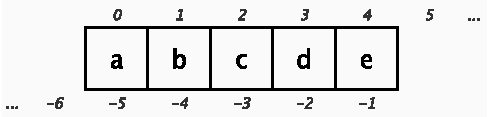
\includegraphics[width=0.6\linewidth]{img/slicing.pdf}		
	\end{figure}
\end{frame}

%%%%%%%%%%%%%%%%%%%%%%%%%%%%%%%%%%%%%%%%%%%%%%%%%%%%%%%%%%%%%%%%%%%%%%%%%%%%%
\begin{frame}[fragile]{Lists - Slicing [start:end]}

	\vspace*{-0.1cm}
	\begin{figure}[!h]
		\centering
		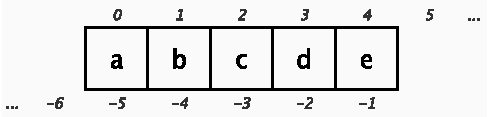
\includegraphics[width=0.6\linewidth]{img/slicing.pdf}		
	\end{figure}

	\vspace*{-0.3cm}
	\pause
	Syntax \small{\texttt{[start:end]}}
	
	\pause
	\begin{pythoncode}
		>>> a[2:4]  # Step = 1.
		['c', 'd']
	\end{pythoncode}

	\pause
	\begin{pythoncode}
		>>> a[2:]  # End is implicit - up to the last item (incl.)
		['c', 'd', 'e']
	\end{pythoncode}

	\pause
	\begin{pythoncode}
		>>> a[:3]  # Start is implicit - from the first item (incl.)
		['a', 'b', 'c']
	\end{pythoncode}

	\pause
	\begin{pythoncode}
		>>> a[1:-1]  # All, but the first and the last.
		['b', 'c', 'd']
	\end{pythoncode}		
\end{frame}


	
%%%%%%%%%%%%%%%%%%%%%%%%%%%%%%%%%%%%%%%%%%%%%%%%%%%%%%%%%%%%%%%%%%%%%%%%%%%%%
\begin{frame}[fragile]{Lists - Slicing [start:end:step]}
	
	\vspace*{-0.1cm}
	\begin{figure}[!h]
		\centering
		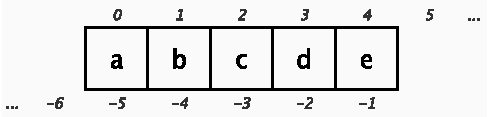
\includegraphics[width=0.6\linewidth]{img/slicing.pdf}		
	\end{figure}

	\vspace*{-0.3cm}
	\pause
	Syntax \small{\texttt{[start:end:step]}}
	
	\pause
	\begin{pythoncode}
		>>> a[1:5:2]  # Every second letter.
		['b', 'd']
	\end{pythoncode}
	
	\pause
	\begin{pythoncode}
		>>> a[4:1:-2]  # Negative step -> going backwards.
		['e', 'd', 'c']
	\end{pythoncode}
	
	\pause
	\begin{pythoncode}
		>>> a[::]  # Implicit start=0, end=5, step=1
		['a', 'b', 'c', 'd', 'e']
	\end{pythoncode}
	
	\pause
	\begin{pythoncode}
		>>> a[4:2:1]  # No valid index in the range.
		[]
	\end{pythoncode}		
\end{frame}


%%%%%%%%%%%%%%%%%%%%%%%%%%%%%%%%%%%%%%%%%%%%%%%%%%%%%%%%%%%%%%%%%%%%%%%%%%%%%
\begin{frame}[fragile]{Dictionaries}

    \begin{itemize}
        \item \pause Unordered set of (\emph{key, value}) pairs
        \item \pause Keys must be immutable (numbers, strings, tuples)
    \end{itemize}

    \pause

    \begin{pythoncode}
        >>> dict = {'name': 'Alice', 'age': 25}
    \end{pythoncode}

    \pause

    \begin{pythoncode}
        # Retrieve entry
        >>> dict['age']
        25
    \end{pythoncode}

    \pause

    \begin{pythoncode}
        # Add or change entry
        >>> dict['city'] = 'Lausanne'

        # Delete entry
        >>> del dict['age']
    \end{pythoncode}

    \pause

    \begin{pythoncode}
        >>> dict
        {'name': 'Alice', 'city': 'Lausanne'}
    \end{pythoncode}

\end{frame}

%%%%%%%%%%%%%%%%%%%%%%%%%%%%%%%%%%%%%%%%%%%%%%%%%%%%%%%%%%%%%%%%%%%%%%%%%%%%%

\begin{frame}[fragile]{Dictionaries}

    \begin{pythoncode}
        # Test if key exists
        >>> 'name' in dict
        True
    \end{pythoncode}

    \pause

    \begin{pythoncode}
        # Get list of keys
        >>> dict.keys()
        dict_keys(['name', 'city'])
    \end{pythoncode}

    \pause

    \begin{pythoncode}
        # Get list of values
        >>> dict.values()
        dict_values(['Alice', 'Lausanne'])
    \end{pythoncode}

\end{frame}

%%%%%%%%%%%%%%%%%%%%%%%%%%%%%%%%%%%%%%%%%%%%%%%%%%%%%%%%%%%%%%%%%%%%%%%%%%%%%

\begin{frame}[fragile]{Dictionaries - Map comprehensions}

    TODO

\end{frame}

%%%%%%%%%%%%%%%%%%%%%%%%%%%%%%%%%%%%%%%%%%%%%%%%%%%%%%%%%%%%%%%%%%%%%%%%%%%%%

\begin{frame}[fragile]{Tuples}

    \begin{pythoncode}
        # Assignment / packing
        >>> tuple = 123, 'abc', 1+5j
    \end{pythoncode}

    \pause

    \begin{pythoncode}
        # Immutable!
        >>> tuple[1] = 'xyz'
        Traceback (most recent call last):
          File "<stdin>", line 1, in <module>
        TypeError: 'tuple' object does not support item assignment
    \end{pythoncode}

    \pause

    \begin{pythoncode}
        # Unpacking
        u, v, w = tuple
    \end{pythoncode}

\end{frame}

%%%%%%%%%%%%%%%%%%%%%%%%%%%%%%%%%%%%%%%%%%%%%%%%%%%%%%%%%%%%%%%%%%%%%%%%%%%%%
%%%%%%%%%%%%%%%%%%%%%%%%%%%%%%%%%%%%%%%%%%%%%%%%%%%%%%%%%%%%%%%%%%%%%%%%%%%%%
%%%%%%%%%%%%%%%%%%%%%%%%%%%%%%%%%%%%%%%%%%%%%%%%%%%%%%%%%%%%%%%%%%%%%%%%%%%%%

\section{Functions}

%%%%%%%%%%%%%%%%%%%%%%%%%%%%%%%%%%%%%%%%%%%%%%%%%%%%%%%%%%%%%%%%%%%%%%%%%%%%%

\begin{frame}[fragile]{Functions}

    Simple function definition:

    \begin{pythoncode}
        >>> def f(a, b):
        ...     return a * b

        >>> f(3, 5)
        15
    \end{pythoncode}

    \pause

    Optional arguments and multiple return values:

    \begin{pythoncode}
        >>> def g(a, b, c=0):
        ...     return a*b - c, a*b + c
        >>> g(3, 5)
        (15, 15)

        # Using tuple unpacking again
        >>> a, b = g(2, 5, 6)  # equivalent to g(2, 5, c=6)
        >>> print(a, b)
        4, 16
    \end{pythoncode}

\end{frame}

%%%%%%%%%%%%%%%%%%%%%%%%%%%%%%%%%%%%%%%%%%%%%%%%%%%%%%%%%%%%%%%%%%%%%%%%%%%%%

\begin{frame}[fragile]{Function - Arguments}

    \begin{itemize}
        \item Arguments are passed as values
        \item \pause Be careful of sneaky bugs!
    \end{itemize}

    \pause

    \begin{pythoncode}
        >>> def h(scalar, array):
        ...     scalar = 9.0
        ...     array[1] = 13

        >>> a = 5.0; l = [1, 2, 3]
        >>> h(a, l)
        >>> print(a, l)
        5.0 [1, 13, 3]
    \end{pythoncode}

    \begin{itemize}
        \item \pause \texttt{l} is actually a reference (passed as an argument)!
    \end{itemize}

\end{frame}

%%%%%%%%%%%%%%%%%%%%%%%%%%%%%%%%%%%%%%%%%%%%%%%%%%%%%%%%%%%%%%%%%%%%%%%%%%%%%
%%%%%%%%%%%%%%%%%%%%%%%%%%%%%%%%%%%%%%%%%%%%%%%%%%%%%%%%%%%%%%%%%%%%%%%%%%%%%
%%%%%%%%%%%%%%%%%%%%%%%%%%%%%%%%%%%%%%%%%%%%%%%%%%%%%%%%%%%%%%%%%%%%%%%%%%%%%

\section{Control Flow}

%%%%%%%%%%%%%%%%%%%%%%%%%%%%%%%%%%%%%%%%%%%%%%%%%%%%%%%%%%%%%%%%%%%%%%%%%%%%%

\begin{frame}[fragile]{Control Flow - Conditional Statements}

    \begin{pythoncode}
        >>> 25
        >>> if x < 0:
        ...     print("Negative")
        ... elif x == 0:
        ...     print("Zero")
        ... else:
        ...     print("Positive")
        ...
        Positive

    \end{pythoncode}

    \begin{itemize}
        \item \pause No parenthesis, no braces
        \item \pause Be careful of indentation
    \end{itemize}

\end{frame}

%%%%%%%%%%%%%%%%%%%%%%%%%%%%%%%%%%%%%%%%%%%%%%%%%%%%%%%%%%%%%%%%%%%%%%%%%%%%%

\begin{frame}[fragile]{Control Flow - Loops}

    Iterate over lists:

    \begin{pythoncode}
        >>> for x in ['a', 'b']:
        ...     print(x)

        a
        b
    \end{pythoncode}

    \pause

    \begin{pythoncode}
        >>> i = 0
        >>> while i < 4:
        ...     # ...
        ...     i += 1
    \end{pythoncode}

    Equivalent, but more concise:

    \begin{pythoncode}
        >>> for i in range(4):
        ...     # ...
    \end{pythoncode}

\end{frame}

%%%%%%%%%%%%%%%%%%%%%%%%%%%%%%%%%%%%%%%%%%%%%%%%%%%%%%%%%%%%%%%%%%%%%%%%%%%%%

\begin{frame}[fragile]{Control Flow - Loops}

    Special functions for lists:

    \begin{pythoncode}
        >>> for idx, val in enumerate(['a', 'b']):
        ...     print(idx, val)

        0 a
        1 b
    \end{pythoncode}

    \pause

    ... and dictionaries:

    \begin{pythoncode}
        >>> dict = {'name': 'Alice', 'age': 25}
        >>> for key, val in dict.items():
        ...     print(key, val)

        name Alice
        age 25
    \end{pythoncode}
\end{frame}

%%%%%%%%%%%%%%%%%%%%%%%%%%%%%%%%%%%%%%%%%%%%%%%%%%%%%%%%%%%%%%%%%%%%%%%%%%%%%
%%%%%%%%%%%%%%%%%%%%%%%%%%%%%%%%%%%%%%%%%%%%%%%%%%%%%%%%%%%%%%%%%%%%%%%%%%%%%
%%%%%%%%%%%%%%%%%%%%%%%%%%%%%%%%%%%%%%%%%%%%%%%%%%%%%%%%%%%%%%%%%%%%%%%%%%%%%

\section{Misc}

%%%%%%%%%%%%%%%%%%%%%%%%%%%%%%%%%%%%%%%%%%%%%%%%%%%%%%%%%%%%%%%%%%%%%%%%%%%%%

\begin{frame}[fragile]{Arithmetic operators}

    \begin{pythoncode}
        # +, -, /, //, *, **
        >>> 1 + 2
        3
    \end{pythoncode}

    \pause

    Floating point vs. integer division:

    \begin{pythoncode}
        >>> 2 / 3
        0.6666666666666666

        >>> 2 // 3
        0
    \end{pythoncode}

    \pause

    Exponentiation:

    \begin{pythoncode}
        >>> 2 ** 3
        8
    \end{pythoncode}
\end{frame}

%%%%%%%%%%%%%%%%%%%%%%%%%%%%%%%%%%%%%%%%%%%%%%%%%%%%%%%%%%%%%%%%%%%%%%%%%%%%%

\begin{frame}[fragile]{Boolean operators}

    \begin{pythoncode}
        >>> True and False
        False
        >>> True or False
        True
        >>> not False
        True
    \end{pythoncode}

    \pause

    \begin{pythoncode}
        # Short-circuiting behaviour
        >>> def fun(i):
        ...     print("executed")
        ...     return i

        >>> True or fun(1)
        True
    \end{pythoncode}

\end{frame}

%%%%%%%%%%%%%%%%%%%%%%%%%%%%%%%%%%%%%%%%%%%%%%%%%%%%%%%%%%%%%%%%%%%%%%%%%%%%%

\begin{frame}[fragile]{Console output}

    \begin{pythoncode}
        >>> print("Hello World!")
        Hello World!
    \end{pythoncode}

    \pause

    Formatted strings (similar to \texttt{printf} in C):

    \begin{pythoncode}
        >>> print("Int: %d, Float: %f, String: %s" % (5, 3.14, 'foo'))
        Int: 5, Float: 3.140000, String: foo
    \end{pythoncode}

\end{frame}

%%%%%%%%%%%%%%%%%%%%%%%%%%%%%%%%%%%%%%%%%%%%%%%%%%%%%%%%%%%%%%%%%%%%%%%%%%%%%

\begin{frame}[fragile]{Packages}

    Load more functionality from (external) packages / files:

    \begin{pythoncode}
        >>> import numpy
        >>> numpy.pi
        3.141592653589793
    \end{pythoncode}

    \pause

    Attention: This overwrites any prior definition of \texttt{pi}!
    \begin{pythoncode}
        >>> from numpy import pi
        >>> pi
        3.141592653589793
    \end{pythoncode}

    \pause

    Often a good ideas to keep things in their own namespaces instead:
    \begin{pythoncode}
        >>> import numpy as np
        >>> np.pi
        3.141592653589793
    \end{pythoncode}

\end{frame}

%%%%%%%%%%%%%%%%%%%%%%%%%%%%%%%%%%%%%%%%%%%%%%%%%%%%%%%%%%%%%%%%%%%%%%%%%%%%%
\begin{frame}[fragile]{More on References, Shallow/Deep Copy}
	
	\begin{itemize}
		\item \pause Everything is \textbf{object} in Python.
		\item \pause Variable stores only \textbf{reference} to the underlying object!
		\item \pause Assigning one variable to another performs \textbf{shallow copy}.
	\end{itemize}
	
	\pause
	\begin{pythoncode}
		>>> A = [1, 2, 3]
		>>> B = array_A
		>>> B[1] = 0
		>>> print(A)
		[1, 0, 3]
	\end{pythoncode}
	
	\begin{itemize}
		\item \pause Module \small{\texttt{copy}} can perform \textbf{deep copy}.
	\end{itemize}
	\begin{pythoncode}
		>>> import copy
		...
		>>> B = copy.copy(A)
		>>> B[1] = 0
		>>> print(A)
		[1, 2, 3]
	\end{pythoncode}
\end{frame}

%%%%%%%%%%%%%%%%%%%%%%%%%%%%%%%%%%%%%%%%%%%%%%%%%%%%%%%%%%%%%%%%%%%%%%%%%%%%%

\begin{frame}[fragile]{References}

    \begin{itemize}
        \item Documentation\\
            \url{https://docs.python.org/3/}
        \item \pause Official python3 tutorial:\\
            \url{https://docs.python.org/3.1/tutorial/index.html}
        \item \pause All built-in functions\\
        	\url{https://docs.python.org/3/library/functions.html}
        \item \pause ...

    \end{itemize}

\end{frame}

\end{document}
